\documentclass[10pt,letterpaper]{article}

\usepackage{cogsci}
\usepackage{pslatex}
\usepackage{pdfsync}
\usepackage{apacite}
\usepackage{amsmath}
\usepackage{graphicx}
\usepackage{topcapt}
\usepackage{color}
%\usepackage{setspace}
%\singlespacing


\title{A Pragmatic Account of the Processing of Negative Sentences}
\author{{\large \bf Ann E. Nordmeyer} \\ \texttt{anordmey@stanford.edu}\\ Department of Psychology \\ Stanford University \\ 
\And {\large \bf Michael C. Frank} \\ \texttt{mcfrank@stanford.edu} \\ Department of Psychology \\ Stanford University \\ }

%\affiliation{Stanford University}

%\abstract{Put Abstract Here.}

%\vspace{3.0ex}

%\noindent Please address correspondence to: Ann E. Nordmeyer, Department of Psychology, Stanford University, 450 Serra Mall, Building 420 (Jordan Hall), Stanford, CA 94305, email: \texttt{anordmey@stanford.edu}.}

%shorttitle{FYP Proposal}
%\rightheader{FYPP}
%\leftheader{A. E. Nordmeyer}

\begin{document}
\maketitle

\begin{abstract}

ABSTRACT

testing git.  

\textbf{Keywords:} 
Negation; sentence processing; pragmatics
\end{abstract}

%%%%%%%%% INTRO %%%%%%%%% 
\section{Introduction}

I am completely lost as to how to start this paper :( :( :(

There is a consistent finding in the literature on negation that participants are slower to evaluate sentences containing a negative element  \cite{hclark1972, carpenter1975, just1971, just1976}.  For example, Clark and Chase (1972) asked participants to compare positive or negative sentences to simple pictures which either matched or did not match the sentences.  Participants were overall slower to respond to negative sentences.  Furthermore, they found an interaction between the type of sentence and the truth of the sentence, with participants responding fastest to true positive sentences and \emph{slowest} to true negative sentences.  This work has been taken as evidence for a propositional view of negation, in which a negative sentence is represented as the denial of an affirmative proposition, leading to greater processing time for negative as opposed to positive sentences. 

The finding that negative sentences take longer to process than positive sentences has been replicated in other paradigms as well.  Electroencephalography studies have shown that semantically unexpected/false sentences such as ``a robin is a truck'' elicit a more negative peak at the N400 compared to sentences such as ``a robin is a bird''.  However, sentences such as ``a robin is not a truck'' produce a greater N400 response than sentences such as ``a robin is not a bird'', suggesting that the negative element ``not'' is not processed immediately (\citeNP{fischler1983}, see also \citeNP{ludtke2008}).  Similar results have been found using probe-recognition tasks.  For example, the sentence ``The door was open'' primes recognition of  a matching picture (an open door) compared to a mismatching picture (a closed door) after 750 ms delay, whereas negative sentences such as ``The door was not open'' do not prime the matching picture (a closed door) until a 1000 ms delay.  (\citeNP{kaup2006}, see also \citeNP{kaup2003, hasson2006}).  Although there is some disagreement about the nature of these representations (e.g. as the denial of a proposition (see \citeNP{hclark1972}), or a mental model of the negated and actual state of affairs (see \citeNP{kaup2003}), this work collectively suggests that negative sentences are more difficult to process than positive sentences.  
  
There is a critical difference, however, between evaluating sentences presented without any context in a laboratory setting and comprehending speech in the real world. According to Grice's cooperative principle \cite{grice1975}, speakers should produce utterances that are appropriately informative, relevant, and unambiguous.  Negative sentences presented without any contextual support often violate this principle.  If my friend asks me what I did this week, and I respond ``I didn't buy a car'', my contribution to the conversation is neither relevant nor informative.  The fact that unsupported negative utterances are generally rated as more ambiguous than unsupported affirmative utterances has been documented experimentally \cite{glenberg1999}.  In general, negative utterances are produced in contexts where there is some \emph{expectation} that the speaker wishes to negate.  For example, if my friend knows that I have been in the market for a new car, then she may be asking about my week because she expects I bought a new car, and my statement ``I didn't buy a car'' becomes relevant and informative.  

Noting that denials are generally produced in response to a violation of expectations, Wason (1965) designed a study to examine whether pragmatic constraints such as context would affect how participants responded to negative sentences.  Participants viewed stimuli consisting of 8 colored dots, in which 7 dots were one color and 1 dot was a different color.  Participants were asked to describe the stimuli, and then evaluate positive and negative sentences about the stimuli.  Wason found that when participants' descriptions of the stimuli highlighted the fact that one of the dots was an exception to the rule, they were faster to evaluate negative sentences about the ``odd'' dot.  Additional work has shown that when participants read sentences that set up a supportive context, reading times for negative sentences are reduced \cite{glenberg1999}, and false positive and false negative sentences show similar N400 responses when the negative sentences are pragmatically licensed \cite{nieuwland2008}.  Children are also sensitive to context effects when processing negative sentences, responding faster to respond to negative sentences about a toy that is different from other toys in the group \cite{devilliers1975}.

Some researchers have found that some contexts are more effective than others at facilitating the processing of negative sentences.  In one such study, contexts which explicitly mentioned or strongly implied the negated characteristic were more effective at reducing reading times of negative sentences compared to contexts which did not mention the relevant characteristic \cite{ludtke2006}.  Critically, these contexts did not have a significant effect on the reading times for positive sentences.  In addition, a mouse-tracking study conducted by Dale and Duran (2011) \nocite{dale2011} found that enhanced contexts lead to significantly smoother mouse trajectories when selecting whether a sentence was true or false, but simple one-sentence contexts did not have an effect.  This work suggests that there is some graded effect of context, with some types of context having a greater effect on negation processing than others, though few studies have thoroughly examined the effect of the strength of the context.

Studies of the effects of pragmatics on linguistic processing exist in other domains as well.  For example, extensive research has been conducted on the processing of scalar implicatures, such as the inference made by listeners that the word "some" excludes the possibility "all", even though semantically the word "some" can encompass "all".  Work by Huang and Snedeker (2009, 2011) \nocite{huang2009, huang2011} suggests that there is a gap between semantic and pragmatic processing, with participants taking significantly longer to resolve referential ambiguity when the resolution involves computing a pragmatic implicature (i.e. some = not all).  However, other work using a similar paradigm suggests that these pragmatic inferences are computed rapidly \cite{grodner2010}.  Degen and Tanenhaus (how to cite?) propose that slow reaction times to compute the scalar implicature for ``some'' may be due to uncertainty about the "question under discussion'' (QUD) \cite{roberts1996}.  This proposal may be relevant to the different processing times seen for negative sentences.  Tian et. al (2010) \nocite{tian2010} found negative constructions of the form ``Eric didn't iron his shirt'' lead participants to respond faster to images of an ironed shirt compared to a wrinkled shirt (consistent with e.g. \citeNP{kaup2006}), negative sentences such as ``It was Eric who didn't iron his shirt'' resulted in the opposite pattern (e.g. faster responses to a wrinkled shirt).  This was interpreted as evidence that the first construction leads to the accommodation of a positive QUD (``Did Eric iron his shirt?''), while the second construction leads to the accommodation of a negative QUD (``Who didn't iron his shirt?'').  Further exploration of the ways that context effects the processing of negative sentences could further our understanding not only of negation, but of how pragmatics can influence sentence processing more generally.  

This paper examines the possibility of a pragmatic account of negation comprehension.  We begin by replicating the finding that context facilitates the processing of negative sentences in a sentence verification task, using visual contexts to set up expectations about the base rate of a certain characteristic (Study 1).  We then explore the effect of the strength of the context by varying that base rate parametrically (Studies 2 and 3).  In order to understand how context might be having an effect on reaction times to evaluate negative sentences, we test the possibility that participants' expectations of how a speaker would describe a given picture are related to processing times (Study 4).  Finally, we attempt to model this relationship between speaker expectations and reaction time, calculating the probability that a speaker would produce an utterance given a certain context to create a model of pragmatic surprisal (see \citeNP{levy2008}, \citeNP{frank2012}).  

\section{Study 1: Context vs. No Context}
Study 1 replicates the finding that negative sentences take adults longer to evaluate than positive sentences when presented without any context \cite{hclark1972, carpenter1975, just1971, just1976}, and further examines the effect of visual contexts on the processing of negative sentences \cite{wason1965}.  The study was conducted using Amazon's Mechanical Turk website, an online crowd-sourcing platform for conducting survey research, and was programmed using Javascript, allowing us to collect reaction times for participants' responses.  CITE OTHER PAPER ABOUT RT ON TURK.  Participants viewed positive and negative sentences such as ``Bob has/has no apples'' along with pictures of people who were either holding the target item (e.g. ``apples'') or holding nothing, and were asked to evaluate whether the sentences were true or false.  Half of the participants first viewed a ``context screen'' which showed e.g. three boys standing with apples.  By replicating a known, robust finding from the literature on Mechanical Turk, this study allowed us to determine whether online platforms are appropriate for collecting sensitive measures such as reaction time (should I take this sentence out now that another study has been published - or should I keep it in, since there still hasn't been a lot of work done in this way?).  In addition, previous work examining context effects on the processing of negative sentences required participants to actively engage with the context, either by describing the stimuli \cite{wason1965} or by reading sentences \cite{dale2011, glenberg1999, ludtke2006}.  This study explores whether a passively-viewed visual context is sufficient for facilitating the processing of negative sentences.  (my feeling about this right now is that if we're submitting this to psych science, I need the motivation for this study to be catchier.  But the truth is, this study in itself isn't very novel - it is the last two that are interesting.  How should I introduce this without making this research sound "incremental")

\subsection{Method}

\subsubsection{Participants}
100 participants were recruited to participate in an online experiment through Amazon's Mechanical Turk website.  Participants ranged in age from 18-65, with the majority of participants being between 18 and 25 (45 participants).  63 participants were male and 37 were female.  Participation was restricted to individuals in the United States, and participants who indicated that their primary language was something other than English were excluded from analysis.  Participants were paid 30 cents to participate in the study, which took approximately 5 minutes to complete.  

\subsubsection{Stimuli}
\begin{figure}[t]
\begin{center} 
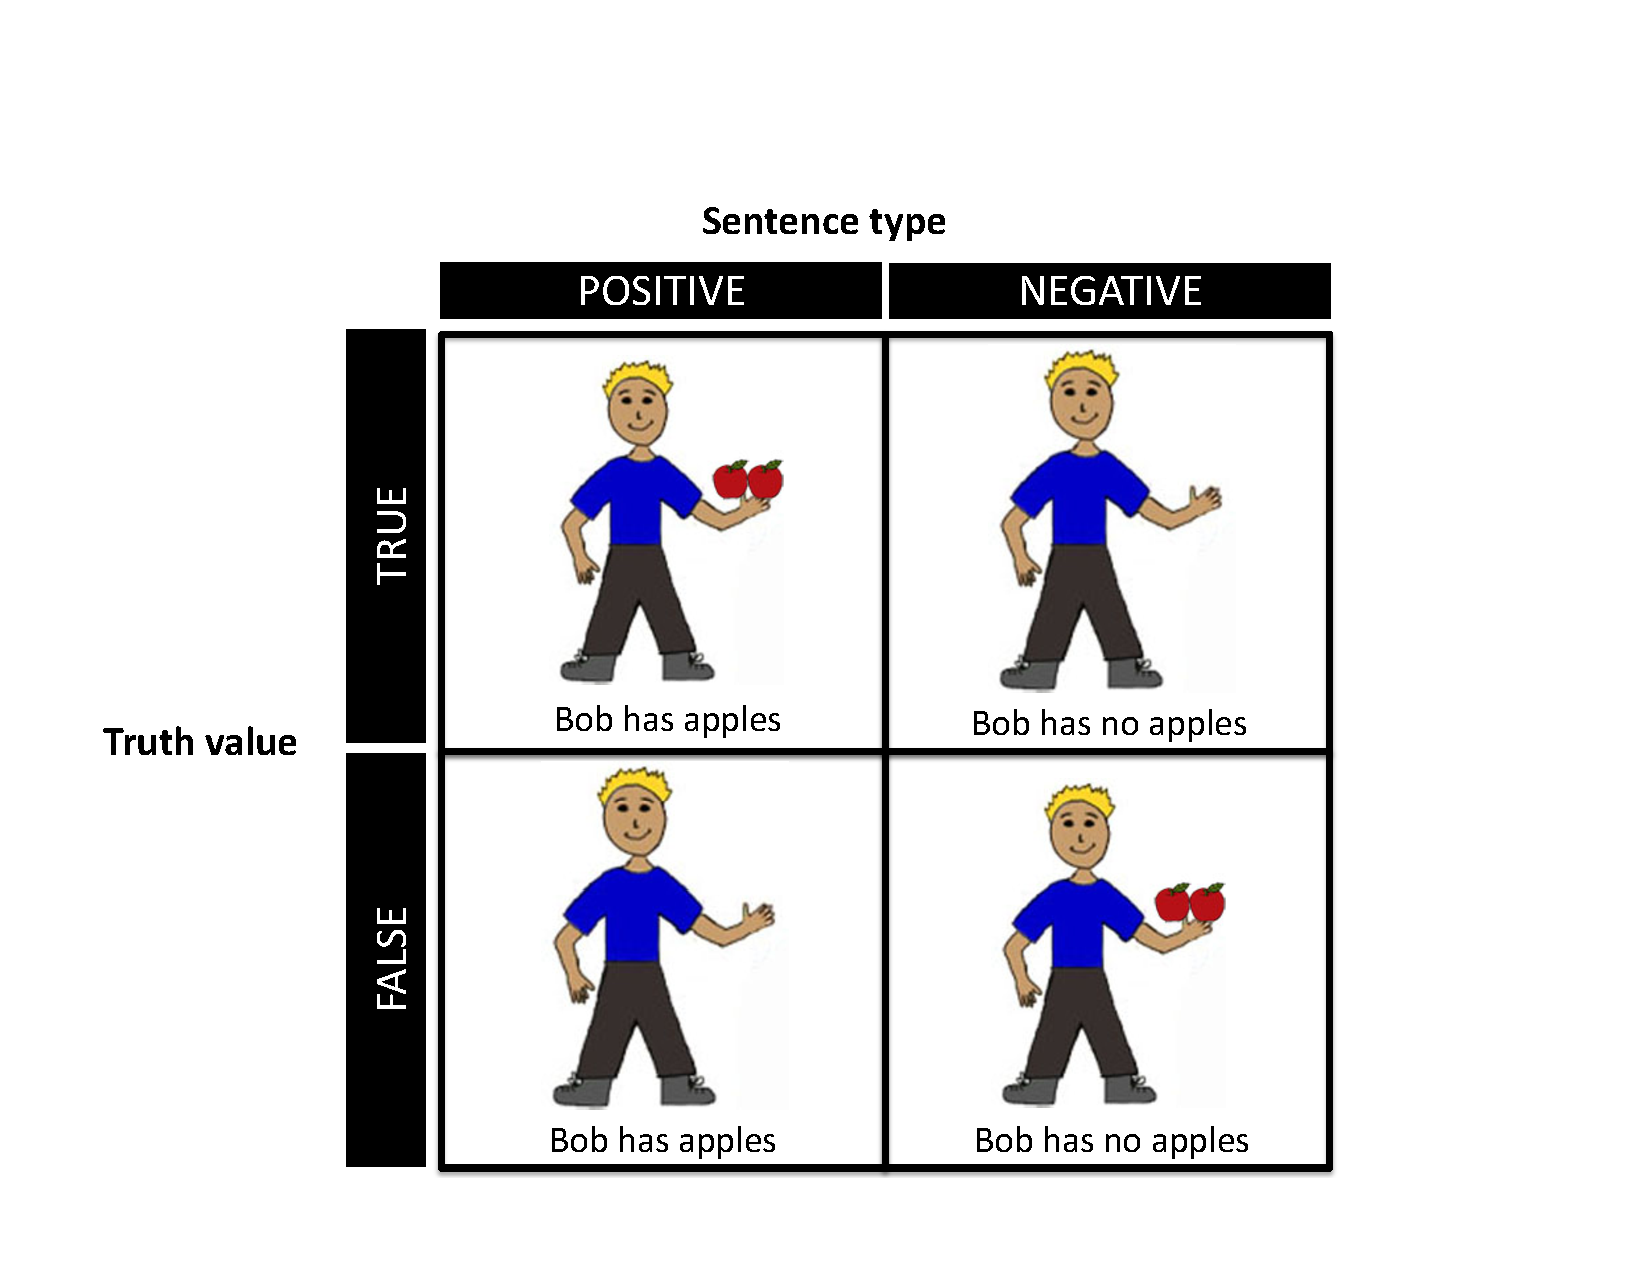
\includegraphics[width=3.25in]{figures/negatron_trialfig.pdf}
\caption{\label{fig:addition_subs} Each participant received four different trial types: true positive, false positive, true negative, false negative. }
\end{center} 
\end{figure}

\begin{figure}[t]
\begin{center} 
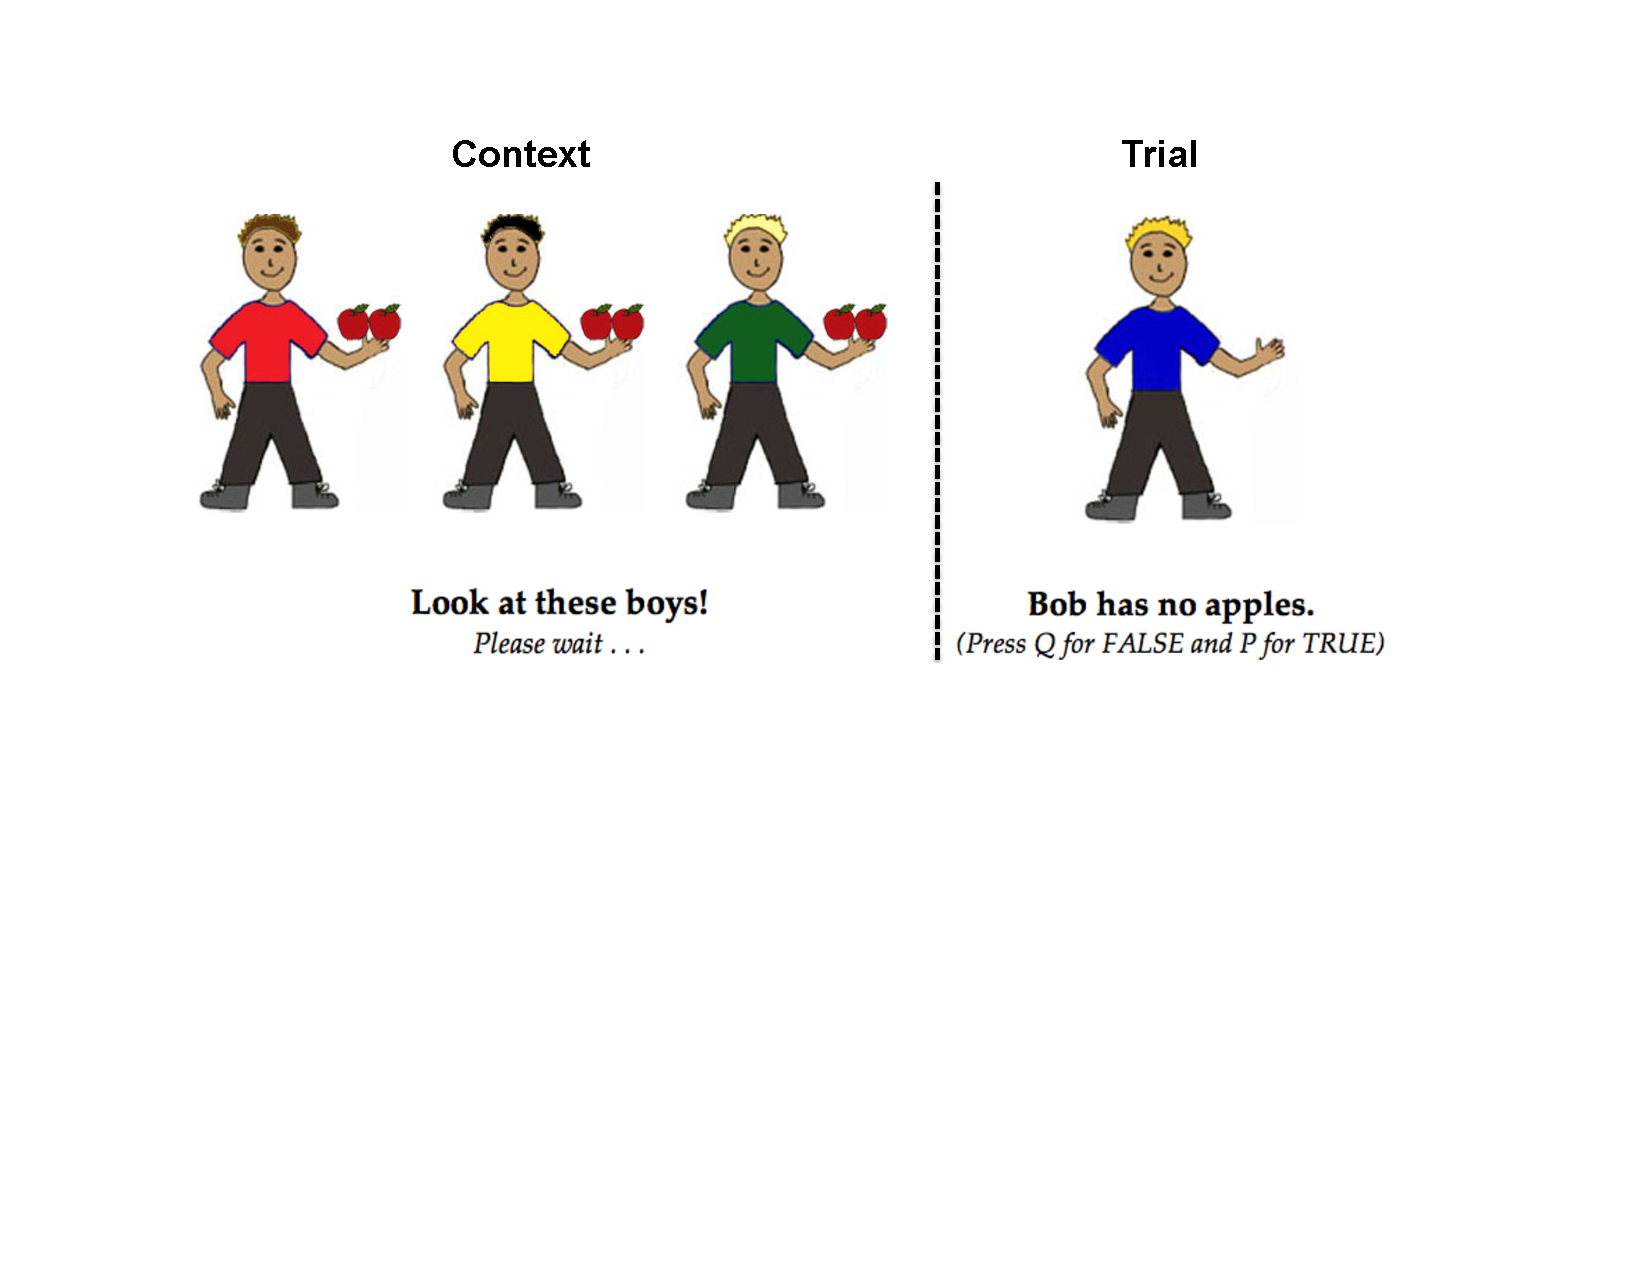
\includegraphics[width=3.25inn]{figures/negatron_trialfig2.pdf}
\caption{\label{fig:addition_subs} An example of a context slide (the 3-person "All" context) and a trial slide (true negative). }
\vspace{-5mm}
\end{center} 
\end{figure}

28 trial items were created in which a character was shown either in possession of two of the same common, recognizable objects (such as apples, buckets, toy cars, cookies, flowers, kites, umbrellas, etc.), or standing alone.  On each trial, beneath the picture, was a sentence of the form ``[NAME] has/has no [ITEM]''.  Half of the sentences were positive and half were negative, and they were paired with pictures such that half were true and half were false.  Lexical negation was used to make the negative sentences match the positive sentences as closely as possible.  The decision to have characters hold two items, rather than one, was made because the negative ``Bob has no apples'' was judged by the authors as more felicitous than ``Bob has no apple''.  

The experiment was fully crossed, with participants receiving 7 true positive, 7 false positive, 7 true negative and 7 false negative sentences over the course of the study.  Trials were presented to participants in a randomized order.

Examples of the four trial types (true positive, false positive, true negative and false negative) can be seen in figure 1.    

Participants were randomly assigned to either the ``No Context'' condition or the ``Context'' condition.  Participants in the ``No Context'' condition saw a blank screen before each trial, while participants in the ``Context'' condition viewed a context slide before each trial.  The context slide showed a picture of three characters, each holding two items.  The characters in the context condition all differed from the trial character and from each other in hair colors and shirt colors.  Beneath the three people was the sentence ``Look at these [boys/girls]!''  An example of a context slide can be seen in figure 2.  


\subsubsection{Procedure}

Participants were first presented with an instructions screen which described the task, followed by 8 practice trials in which participants judged whether a sentence about the color of a character's clothing was true or false.  During the practice trials, if participants answered a question incorrectly a pop-up window informed them that they were incorrect and instructed them to try again.  At the end of the practice, another instructions screen reminded them of the procedure and told them to press space to start the ``game''.  

Before each trial, participants either viewed a blank screen or a context screen, depending on the condition they were assigned to.  In both cases the experiment automatically advanced after 3 seconds.  They then saw a picture and a sentence about that picture, and they were asked to select whether the sentence was true or false by pressing ``Q'' for false or ``P'' for true.  Participants were told to answer and quickly and accurately as possible.  Once participants made their selection by pressing "P" or "Q", they were automatically brought to the next trial after a 500 ms pause.  Participants were instructed to use their left hand to select the ``Q'' key and their right hand to press the ``P'' key, to ensure that they would be able to respond as quickly as possible.  Reaction times, measured as the time from when the pictures/sentence were presented to the moment when the participant made their response, were recorded by the computer 

At the end of the experiment, participants were taken to a screen that collected demographic information.  Participants were required to enter their gender, age, and native language, and then were invited to provide optional comments about the task.  

\subsection{Results}

\begin{table}[t]
\caption{Means and standard deviations of reaction times in milliseconds for each of the four trial types, for each of the two context conditions.}
\begin{center}
\small\addtolength{\tabcolsep}{-5pt}
\begin{tabular}{ r  r  r  r  r } 
\hline
& \multicolumn{2}{c}{\bf{No Context}} & \multicolumn{2}{c}{\bf{Context}} \\
  \bf{Trial Type} & \bf{Mean} & \bf{SD} & \bf{Mean} & \bf{SD} \\ \hline                    
True Positive & 1513 & 618 &  1481 & 692\\
 False Positive & 1713 & 634 &  1564 & 582\\
 True Negative& 1805 & 552 & 1555 & 645\\
  False Negative & 1724 & 561 & 1594 & 622 \\
\hline
\end{tabular}
\end{center}
\end{table}

\begin{figure}
\begin{center} 
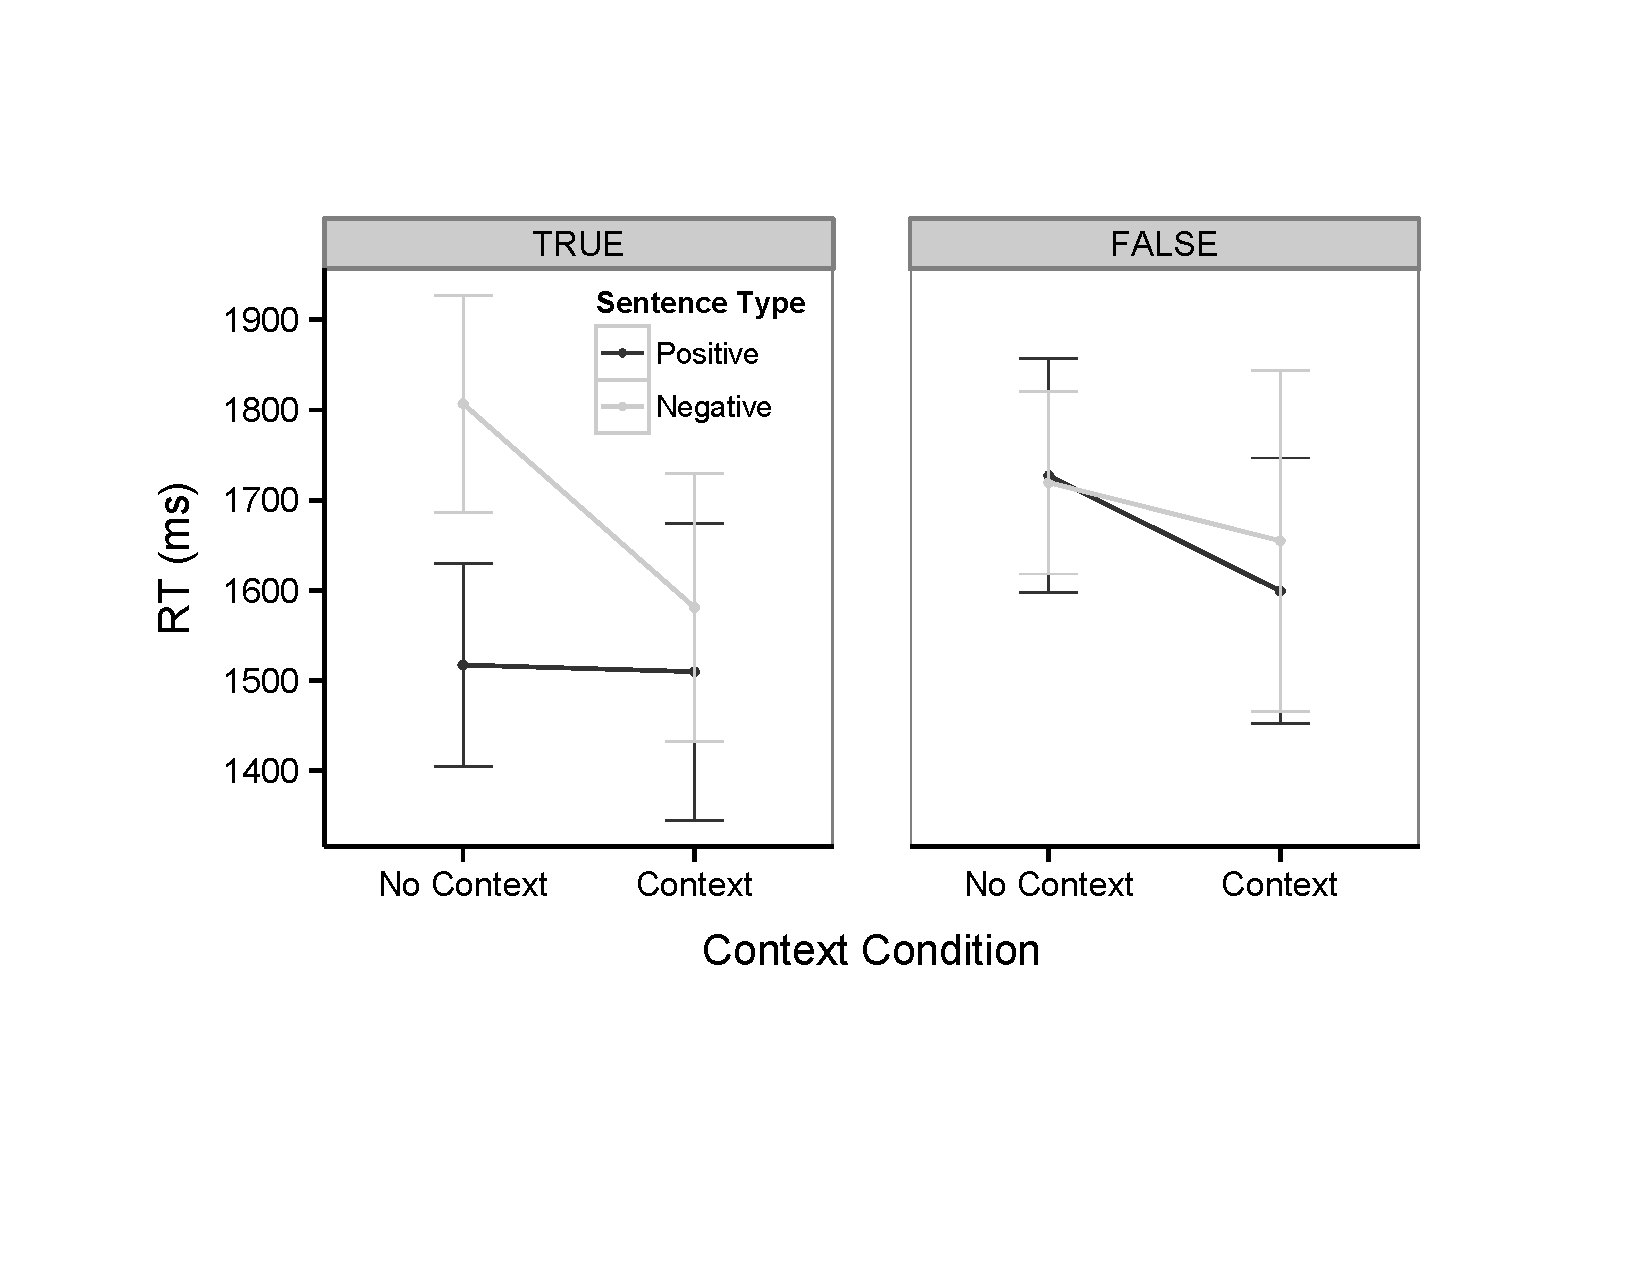
\includegraphics[width=3.25in]{figures/study1_linegraph.pdf}
\caption{\label{fig:addition_subs} Reaction times for each trial type, across different conditions.  Error bars represent the 95\% confidence intervals.}
\end{center} 
\end{figure}

\begin{table*}[t]
\caption{Coefficient estimates from a linear effects model estimating the effects of context condition, sentence type, and response on reaction time, accounting for random effects of participant and item.}
\begin{center}
\small\addtolength{\tabcolsep}{-5pt}
\begin{tabular}{ r  r  r  r  } 
\hline
  \bf{Fixed Effects} & \bf{Coef.} & \bf{Std. Error} & \bf{t value} \\ \hline             
Sentence type(negative) & 9.566 & 47.620 & 0.201\\
Response(true) &  -200.187 & 42.552 & -4.704\\
Context condition(context) & -123.582 & 97.790 & -1.264\\
Trial number & -7.838 & 1.300 & -6.029\\
Sentence type(negative)*Context condition(context) & 21.774 & 65.565 & 0.332\\
Sentence type(negative)*Response(true) & 264.017 & 61.924 & 4.264\\
Context condition(context)*Response(true) &  118.445 & 58.622 & 2.020\\
Sentence type(negative)*Context condition(context)*Response(true) & -231.469 & 85.424 & -2.710\\
\hline
\end{tabular}
\end{center} 
\end{table*}

Study 1 examined the effect of a visual context on the processing of negative sentences.  Previous research led us to expect a main effect of sentence type, with negative sentences incurring greater RTs than positive sentences, as well as a main effect of truth value, with false sentences incurring greater RTs than true sentences, and a sentence type*truth value interaction in the no context condition \cite{hclark1972}.  We hypothesized that participants in the context condition, who first viewed a visual context setting up an expectation (e.g. that boys have apples), would show faster responses to negative sentences than participants in the no context condition.  

Six participants who listed a language other than English as their native language were excluded from analysis.  Seven additional participants were excluded for having participated in a previous iteration of the experiment.  Four participants were excluded for having an overall accuracy of below 80\%.  Thus, data from a total of 83 participants were analyzed.  

Only correct trials were analyzed, due to the well-documented speed-accuracy tradeoff found in measures of reaction time.  Trials with RTs greater than 3 standard deviations from the mean were also excluded from the analysis.  Mean RTs and standard deviations for each of the four trial types are presented in table 1.  A graph of these data can be seen in figure 3.  Looking just at the data for participants in the ``no context'' condition, the effects seen here replicate previous work on the processing of negative sentences \cite{hclark1972, carpenter1975, just1971, just1976}, with negative sentences slower than true sentences, false sentences slower than true sentences, and an interaction between sentence type and response.  However, comparing this to the data from participants in the context condition, there appears to have been a facilitating effect of context, such that participants who first viewed the context slides had lower RTs.  This effect was strongest for true negative sentences.  

A maximal linear mixed effects analysis was conducted to examine the effects of sentence type, response (truth value), and context on log(RT).  Sentence type (positive or negative), response (true or false), and context condition (context or no context) and their interaction as were included as fixed effects, and the model accounted for random intercepts and slopes across participants and items.  (note: is this the best way to report this?  I noticed in Alex stiller's paper he reports two separate models, one for the experimental group and one for the control.  If i split this analysis up into two models, one for no context and one for context, would that make my results easier to interpret?)

\subsection{Discussion}

Study 1 provides further evidence for the effects of context on the processing of negative sentences.  Several previous studies have shown that embedding negative sentences in a supportive linguistic context facilitates the processing of negative sentences \cite{dale2011, glenberg1999, ludtke2006}.  In this study, we presented participants with a visual context that was designed to set up an expectation for what the trial picture might look like.  For example, if participants viewed a context showing three boys holding apples, this sets up an expectation that boys have apples.  We found that viewing these contexts before each trial lead to faster processing of negative sentences, with true negative sentences showing the greatest effect.  

To understand why context had the greatest effect on true negative sentences, consider what a true negative trial looks like to a participant in the no context condition.  These are trials in which the participant has no expectation about what the character might be holding, because no context was provided to set up such an expectation.  The participant would then see a picture of a boy, not holding anything, with the sentence ``Bob has no apples''.  It seems obvious that a sentence such as this would cause participants to falter, since there is no reason for ``apples'' to be mentioned at all.  However, when a participant first views a context such as the one pictured in figure ??, they can form an expectation based on this context that boys hold apples.  Now, when the trial shows a boy with no apples, a sentence such as ``Bob has no apples'' makes sense and can be processed rapidly, because the image violates an expectation that boys should have apples.  

Study 1 contributes to a body of evidence suggesting that negative sentences are more felicitous when they are used to negate an expectation that participants might hold, and that such expectations can be set up by an appropriate context.  In study 2, we examine how participants responses are affected by changing the strength of the expectations set up by the context.  

\section{Study 2: Three-person Context}
While study 1 provides evidence that negative sentences - in particular, true negative sentences - are facilitated by the presence of a context, it does not explain how or why context has this effect.  In order to further examine the effect of context on negation, we quantitatively manipulated the strength of the context, so that some participants saw contexts in which none of the characters were holding items (i.e. all three were empty-handed), some saw contexts in which 1/3 of the characters had items, some saw contexts in which 2/3 of the characters had items, and some saw contexts in which all of the characters had item (as in the ``Context'' condition in study 1).  If one thinks of the contexts as giving participants a glimpse into the ``world'' that each trial exists in, the context gives the participant a small sample of the base rate of what the characters in this ``world'' look like.  By manipulating the base rate of e.g. boys who have apples, we can change peoples' expectations about what the trial character will look like.  If the differences in reaction times between the no context and the context condition in study 1 really are due to the difference in the expectations set up by the context, we should be able to further manipulate reaction times by systematically varying the strength of the expectation set up by the context.  

Recent work by Frank et al. \cite{frank2009, frank2012} has attempted to quantify the pragmatic inferences that adults make when playing simple ``language games''. The assumption underlying the predictions made by these authors is that speakers are informative - that is, they will produce utterances that will pick out smaller subsets of the context, leaving as little ambiguity as possible for the listener.  Regarding the present study, this should predict a linear effect of context on RTs to negative sentences, since ``Bob has no apples'' is not very informative at all when the context contains three boys with no apples - it could apply to any of the boys that the participant has seen.  However, as the context changes and more boys in the context \emph{have} apples, the informativeness of the statement ``Bob has no apples'' increases, because it applies to an increasingly smaller subset of the context.  Study 2 tests this prediction by varying the contexts that different participants see before each trial.  (Note: I wasn't sure what predictions I should make here.  I think originally we did have a prediction that we would find a linear effect.  Do I stick with this as our original hypothesis, or do I frame this study based on what we know now - that it is actually more like a u-shaped relationhip?)



\subsection{Method}

\subsubsection{Participants}
200 participants were recruited to participate in an online experiment through Amazon's Mechanical Turk website.  Participants ranged in age from 18-70, with the majority of participants being between 18 and 25 (84 participants).  129 participants were male and 71 were female.  Participation was restricted to individuals in the United States, and participants who indicated that their primary language was something other than English were excluded from analysis.  Participants were paid 30 cents to participate in the study, which took approximately 5 minutes to complete.  


\subsubsection{Stimuli}
Study 2 used the same 28 trial items and sentence types as those used in Study .  A between-subjects ``context'' factor determined what type of context participants saw.  In the ``none'' context condition, participants saw three characters without any objects.  In the ``one'' context condition, participants saw two characters with nothing and once character holding two of the expected object.  In the ``two'' context condition, participants saw one character with nothing and two characters holding the expected objects.  In the ``all'' context condition, participants saw three characters holding the expected objects (identical to the ``Context'' condition in Study 2).  Beneath the three characters was the sentence ``Look at these [boys/girls]!''  Examples of the None, One, and Two context conditions can be seen in figure 4.  Trial stimuli were identical to the stimuli used in Studies 1 and 2.  

\subsubsection{Procedure}
 The procedure was identical to the procedure in Study 1, with participants randomly assigned to one of the four context conditions.
 
\subsection{Results}

\begin{table}[t]
\caption{Means and standard deviations of reaction times in milliseconds for each of the four trial types, across each of the four contexts.}
\begin{center}
\small\addtolength{\tabcolsep}{-5pt}
\begin{tabular}{ r  r  r  r  r  r  r  r  r} 
\hline
& \multicolumn{2}{c}{\bf{None}} & \multicolumn{2}{c}{\bf{One}}  & \multicolumn{2}{c}{\bf{Two}}  & \multicolumn{2}{c}{\bf{Three}}\\
\hline
  \bf{Trial Type} & \bf{Mean} & \bf{SD} & \bf{Mean} & \bf{SD} & \bf{Mean} & \bf{SD} & \bf{Mean} & \bf{SD} \\ \hline                      
True Positive & 1519 & 578 & 1412 & 612 & 1456 & 543 & 1487 & 592\\
 False Positive & 1685 & 668 & 1526 & 567 & 1489 & 475 & 1610 & 566\\
 True Negative& 1697 & 593 & 1629 & 666 & 1505 & 498 & 1600 & 560\\
  False Negative & 1692 & 604 & 1543 & 602 & 1528 & 525 & 1737 & 672\\
\hline
\end{tabular}
\end{center}
\end{table}

\begin{figure}
\begin{center} 
\includegraphics[width=3.25in]{figures/study2_linegraph.pdf}
\caption{\label{fig:addition_subs} Reaction times for each trial type, across different conditions.  Error bars represent the 95\% confidence intervals.}
\end{center} 
\end{figure}

\begin{table*}[t]
\caption{Coefficient estimates from a linear effects model estimating the effects of context condition (quadratic), sentence type, and response on reaction time, accounting for random effects of participant and item.}
\begin{center}
\small\addtolength{\tabcolsep}{-5pt}
\begin{tabular}{ r  r  r  r  } 
\hline
  \bf{Fixed Effects} & \bf{Coef.} & \bf{Std. Error} & \bf{t value} \\ \hline             
Context(quadratic) &-3.8301 & 9.0699 & -0.42\\
Sentence type(negative) &  -6.1572 & 30.6565 & -0.20\\
Response(true) & -120.6406 &   28.1636 &  -4.28\\
Trial number & -6.7562   &  0.8036  & -8.419\\
Context(quadratic)*Sentence type(negative)&15.3235  &   5.3769  &  2.85\\
Context(quadratic)*Response(true) & 6.1625  &   5.6339  &  1.09\\
Sentence type(negative)*Response(true) &  178.5123 &   42.8571  &  4.17\\
Context(quadratic)*Sentence type(negative)*Response(true) & -26.3395  &   8.0837 &  -3.26\\
\hline
\end{tabular}
\end{center}
\end{table*}


Study 2 examined the effect of manipulating the context in ways that should change participants' expectations about what each trial should look like.  We predicted that there would be an inverse linear effect of context, such that as the number of e.g. boys with apples in the context increased, reaction times to evaluate negative sentences would decrease.  

Seven participants who listed a language other than English as their native language were excluded from analysis.  Fifteen additional participants were excluded for having participated in a previous iteration of the experiment.  Eleven participants were excluded for having an overall accuracy of below 80\%.  Thus, data from a total of 167 participants were analyzed.  

Only correct trials were analyzed, due to the well-documented speed-accuracy tradeoff found in measures of reaction time.  Trials with RTs greater than 3 standard deviations from the mean were also excluded from the analysis.  Mean RTs and standard deviations for each of the four trial types are presented in table 3.  A graph of RTs for each trial type across conditions is presented in figure 5.  

Looking at figure 5, there appears to be a quadratic effect of context on RT, particularly for true negative sentences, such that the ``two'' context has the greatest effect of increasing RTs for these sentences, and RTs for True Negative sentences appear to decrease slightly in the ``all'' context condition.  With context condition coded as a continuous variable, we tested a maximal mixed effects model which examined the effect of sentence type, response, the quadratic effect of context, and the interaction between the three on reaction time.  Effects of participants and items were included as random effects.  In this model, the interaction between context as a quadratic variable and negative sentence types was positive (t=2.85), as was the three-way interaction between a quadratic effect of context, negative sentence types, and true sentences (t=-3.26) (note: does this make sense?), suggesting that the pattern seen in figure 5 is statistically significant.  Estimated coefficients for this model are presented in table 4.  

\subsection{Discussion}
Study 2 was designed to test how the effect of context changes when the strength of the context is quantitatively manipulated.  We hypothesized that the effect of context would increase linearly as the strength of the context increased (i.e. the number of boys with apples in the context).  We found that our manipulation of the context actually produced a quadratic effect, such that a context in which participants saw 2 out of 3 boys holding apples produced the fastest reaction times, while the context in which all 3 boys were holding apples showed slightly increased reaction times.  

The fact that we found a quadratic relationship between context and reaction times to respond to negative sentences was unexpected, but can also be explained in terms of the pragmatics of negationl.  In our original hypothesis, we were considering the surprisal of the \emph{sentence}, ``Bob has no apples''.  However, if you also consider the surprisal of seeing a certain \emph{picture}, the quadratic relationship seen in study 2 begins to make more sense.  In the ``None'' context, seeing the sentence ``Bob has no apples'' is always surprising, because there is no reason to talk about a lack of apples - none of the boys have apples, so attributing this fact to Bob is not informative and it is not relevant to the context.  In the ``one'' context, the sentence ``Bob has no apples'' becomes slightly more relevant, because apples have been introduced to the context, but since the majority of the boys don't have apples, it is still uninformative.  However in the ``two'' condition, now the majority of the boys have apples, making Bob's lack of apples highly relevant and also informative.  This is true in the ``all'' condition as well, but in the ``all'' condition you never see a boy without apples in the context - therefore, it seems that the slight increase in RTs in the ``all'' context could be due to a small amount of surprisal at seeing a boy with nothing, since the expectation is that boys will have apples.  This expectation makes negation in the ``all'' condition felicitous, but could cause a slight increase in RT as the participants encode this unexpected picture.  Thus, the ``two'' condition, which sets up an expectation that the majority of boys have apples while also allowing for other possibilities (i.e. boys with nothing), has the greatest effect on facilitating the processing of negative sentences. 



\section{Study 3: Four-person Context}
blah blah blah

\subsection{Method}

\subsubsection{Participants}
400 participants were recruited to participate in an online experiment through Amazon's Mechanical Turk website.  Participants ranged in age from 18 to over 65, with the majority of participants being between 18 and 25 years old (184 participants).  205 participants were male and 195 were female.  Participation was restricted to individuals in the United States, and participants who indicated that their primary language was something other than English were excluded from analysis.  Participants were paid 40 cents to participate in the study, which took approximately 7 minutes to complete.

\subsubsection{Stimuli}
In study 3, the number of items was increased to 48.  As in study 2, a between-subjects ``context'' factor determined what type of context participants saw.  The contexts were the same as those in study 2, except that each context contained 4 boys and there were therefore 5 context conditions (none, one, two, three, and four).  

\subsubsection{Procedure}
 The procedure was identical to the procedure in studies 1 and 2, with participants randomly assigned to one of the five context conditions.

\subsection{Results and Discussion}


\begin{figure}
\begin{center} 
\includegraphics[width=3.25in]{figures/study3_linegraph.pdf}
\caption{\label{fig:addition_subs} Reaction times for each trial type, across different conditions.  Error bars represent the 95\% confidence intervals.}
\end{center} 
\end{figure}

\begin{figure}
\begin{center} 
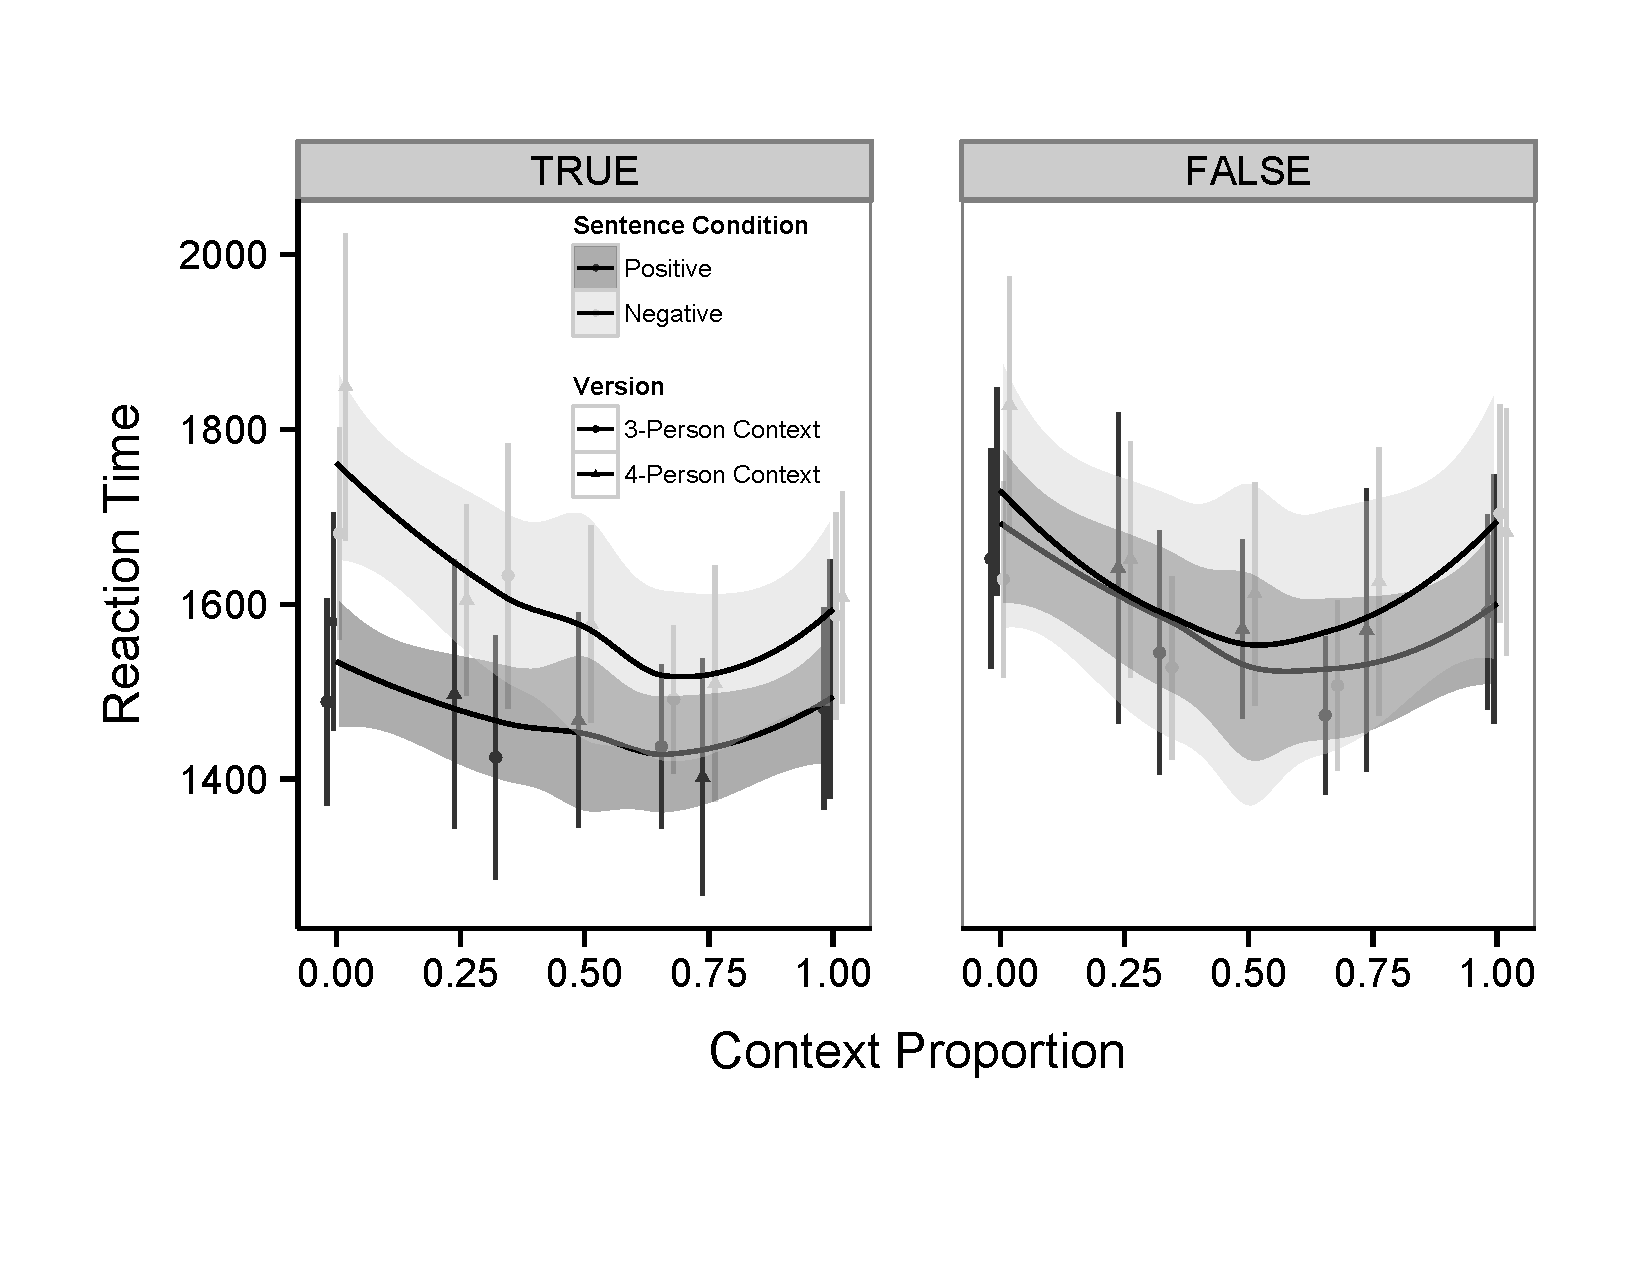
\includegraphics[width=3.25in]{figures/combined_plot.pdf}
\caption{\label{fig:addition_subs} Reaction times for each trial type, across different conditions.  Error bars represent the 95\% confidence intervals.}
\end{center} 
\end{figure}

\begin{table*}[t]
\caption{Coefficient estimates from a linear effects model estimating the effects of context condition (quadratic), sentence type, and response on reaction time, accounting for random effects of participant and item.}
\begin{center}
\small\addtolength{\tabcolsep}{-5pt}
\begin{tabular}{ r  r  r  r  } 
\hline
  \bf{Fixed Effects} & \bf{Coef.} & \bf{Std. Error} & \bf{t value} \\ \hline                     
Context(quadratic) & -5.1314   &  3.9488  & -1.30\\
Sentence type(negative) & 51.5396 &   22.4416   & 2.30\\
Response(true) & -147.4821  &  18.7467 &  -7.87\\
Trial number &-3.4087 &    0.2772 &  -12.30 \\
Context(quadratic)*Sentence type(negative)&  0.1794  &   2.1696  &  0.08\\
Context(quadratic)*Response(true) &  3.3698 &    2.1134  &  1.59 \\
Sentence type(negative)*Response(true) &124.0178 &   28.8466 &   4.30  \\
Context(quadratic)*Sentence type(negative)*Response(true) & -5.8065  &   2.9911  & -1.94\\
\hline
\end{tabular}
\end{center}
\end{table*}

Study 3 explored the U-shaped effect of context on reaction time seen in study 2 by expanding the contexts to include 4 characters and thus creating 5 different context conditions.  We predicted a similar pattern as that seen in study 2, with reaction times decreasing as the number of characters with the target item in the context increased, but with the ``all'' context showing increased reaction times.  

?? participants who listed a language other than English as their native language were excluded from analysis.  ?? additional participants were excluded for having participated in a previous iteration of the experiment.  ??participants were excluded for having an overall accuracy of below 80\%.  Thus, data from a total of ?? participants were analyzed (sorry I didn't have these numbers on-hand - I'll fill these in ASAP, I thought I'd written them down but I'll have to run the R script again to check them).  

Only correct trials were analyzed, due to the well-documented speed-accuracy tradeoff found in measures of reaction time.  Trials with RTs greater than 3 standard deviations from the mean were also excluded from the analysis. A graph of RTs for each trial type across conditions is presented in figure ??.   (I don't have a table of means for this study - I can make one easily, but I'm undecided on how useful it is.  I made the ones for studies 1 and 2 for my FYP, which is why I included them here, but do you think they are just a waste of space and I should only include the graphs?)

Figure 6 shows a similar U-shaped function as the one seen in study 2 - reaction times decrease as the number of boys/girls with the target item increases, but increase again in the ``all condition''.  As before, a maximal mixed effects model was tested, examining the effect of sentence type, response, the quadratic effect of context, and the interaction between the three on reaction time with items and participants as random effects.  The three-way interaction between a quadratic effect of context, negative sentence types, and true sentences was (marginally??) significant (t=-1.94).  Estimated coefficients for this model are presented in table 5.  

A meta-analysis of the data was conducted by pooling together results of both studies, and plotting the results.  In these figures (figure 7 and figure 8), the context condition was plotted on the x-axis as the proportion of characters in the context with the target item, such that 0 = ``none'' context condition and 1 = ``all'' context condition.  Figure 7 shows the standardized difference scores, calculated as (true negative RTs - true positive RTs) / (true negative RTs + true positive RTs) for each subject, then aggregated and standardized within each experiment.  Figure 8 shows the standardized RTs for true positive and true negative sentences in each study.  This graph shows that the U-shaped relationship seen in figure 7 are driven primarily by changes in responses to true negative sentences, while responses to true positive sentences stay fairly consistent across contexts.  (I know I need to say more here about this analysis, but I'm not sure what.  I don't have any statistical analysis to report here - should I?)



\section{Study 4: Measuring Listener Expectations}
Introduce idea of surprisal, levy 2008, pragmatic surprisal, etc. 

\subsection{Method}

\subsubsection{Participants}

\subsubsection{Stimuli}

\subsubsection{Procedure}

\subsection{Results}
\begin{figure}
\begin{center} 
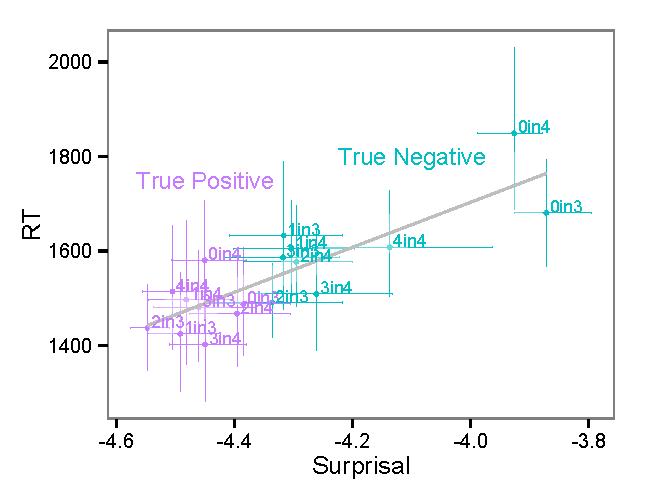
\includegraphics[width=3.25in]{figures/speakerstudy_comparison.pdf}
\caption{\label{fig:addition_subs} Reaction times for each trial type, across different conditions.  Error bars represent the 95\% confidence intervals.}
\end{center} 
\end{figure}

\subsection{Discussion}

\section{Model}

Intro to model: 

Tian et al. suggest that instead of representing the affirmative, listeners represent the QUD.  In many laboratory tasks this involves representing a positive QUD (e.g. in response to the sentence "Mike didn't iron his shirt", the QUD would be "Did Mike iron his shirt?".).  However, other negative sentences presuppose negative QUDs, e.g. "It was Mike who didn't iron his shirt" presupposes "Who didn't iron their shirt?".  

Sections for model???

\begin{figure}
\begin{center} 
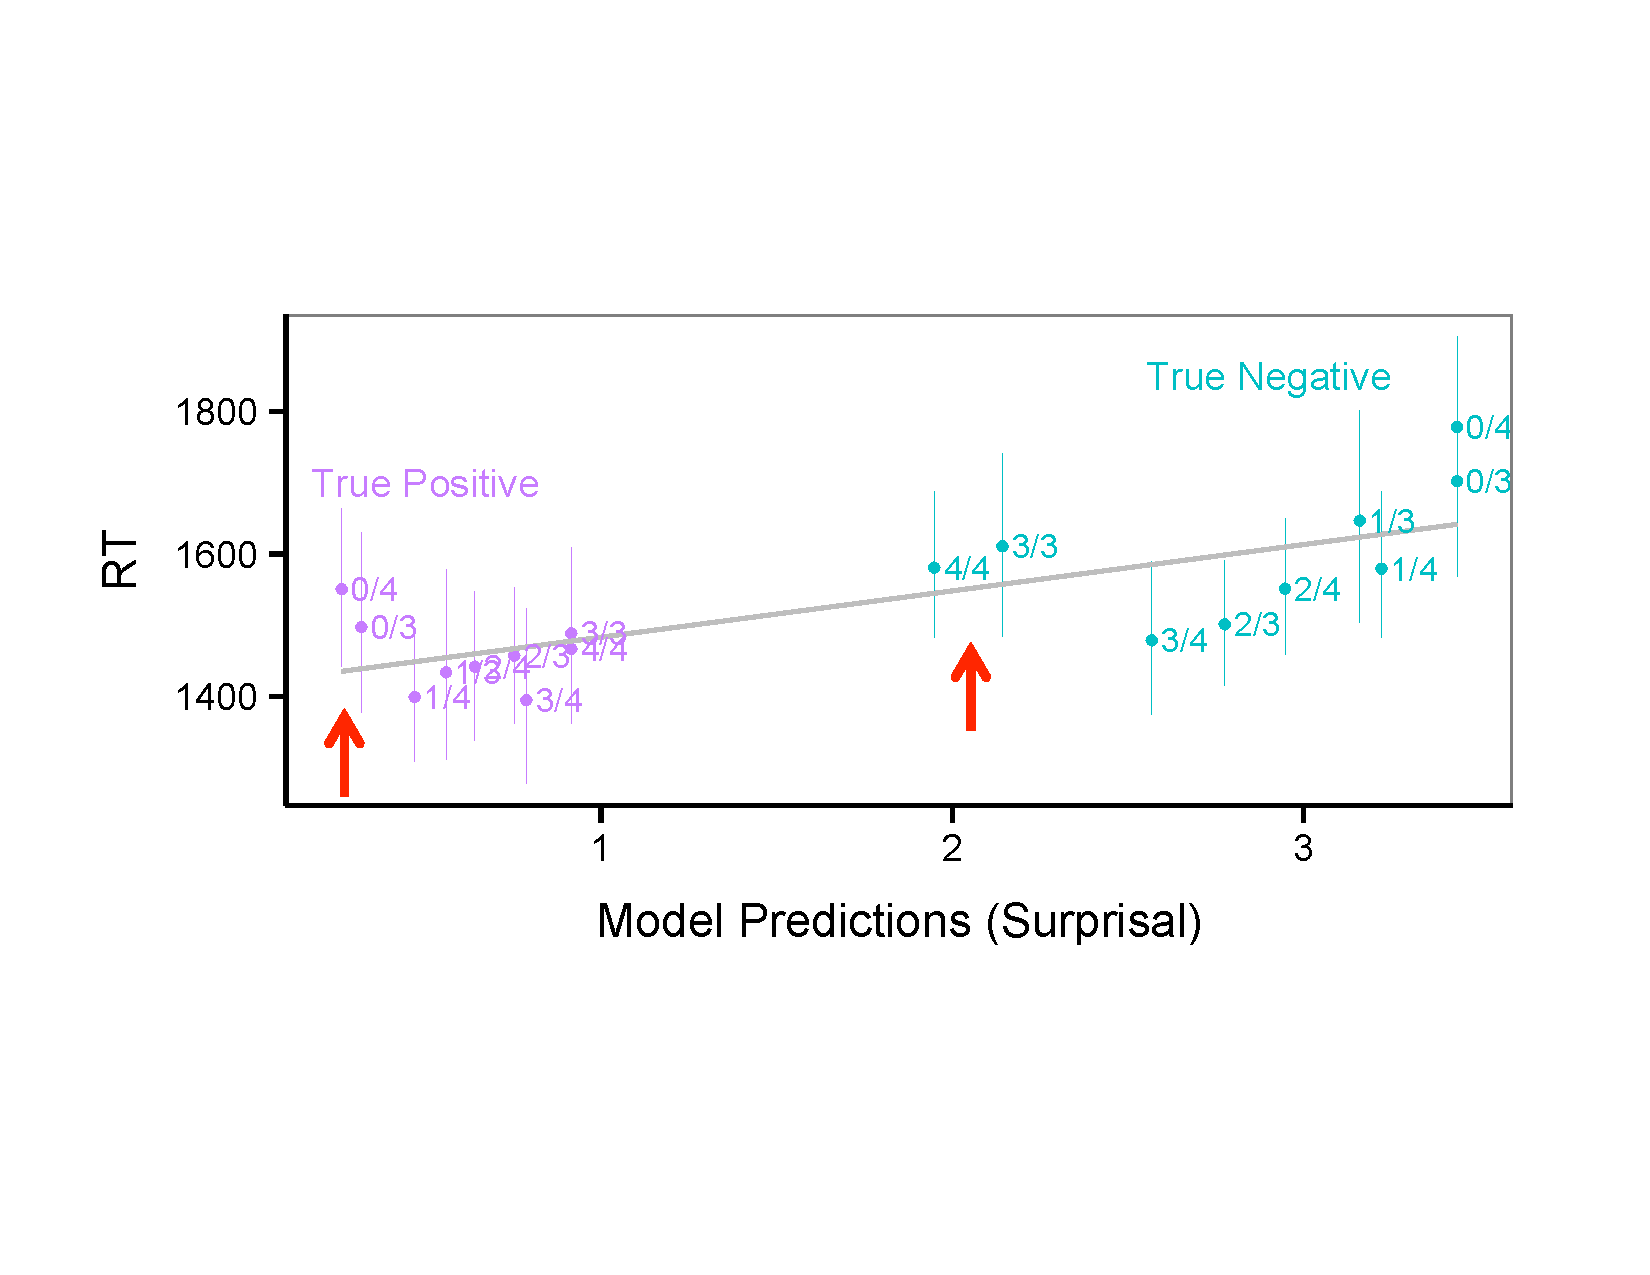
\includegraphics[width=3.25in]{figures/model1_comparison.pdf}
\caption{\label{fig:addition_subs} Reaction times for each trial type, across different conditions.  Error bars represent the 95\% confidence intervals.}
\end{center} 
\end{figure}

\begin{figure}
\begin{center} 
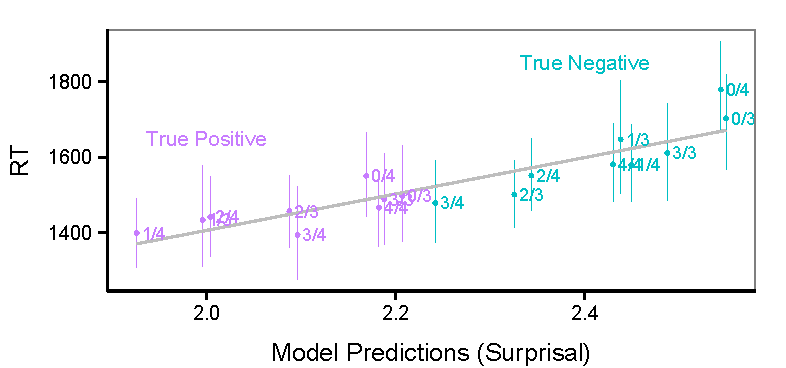
\includegraphics[width=3.25in]{figures/model2_comparison.pdf}
\caption{\label{fig:addition_subs} Reaction times for each trial type, across different conditions.  Error bars represent the 95\% confidence intervals.}
\end{center} 
\end{figure}


\section{General Discussion}
POSSIBLY CITE PEA 1979??


This paper explores the relationship between the processing of negative sentences, and the contexts in which these sentences are presented.  Previous work has shown that although it takes longer to evaluate negative sentences than positive sentences when test sentences are presented with no context \cite{carpenter1975, just1971, just1976, hclark1972}, the presence of a verbal context \cite{dale2011, glenberg1999, ludtke2006} or the process of describing a visual context \cite{wason1965} can facilitate the processing of negative sentences.  This suggests that a pragmatic account of negative sentences is warranted, such that negative sentences are licensed in contexts which set up an expectation which is then violated.  However, the extent to which expectation modulates the processing of negative sentences has not been systematically examined until now.  

In the studies presented here, we quantitatively manipulated the expectation set up by the context by changing the proportion of people in the context who held a certain target item.  We found a quadratic relationship between the proportion of people in the context with the target item and the reaction times to respond to negative sentences.  This effect was most striking in response to true negative sentences, in which participants saw a person holding nothing and saw a sentence such as ``Bob has no apples''.  True positive sentences showed little, if any, effect of context.  

To understand the quadratic effect of context, we must consider how the context alters a participant's expectations about the picture that may appear as well as the likelihood of a negative term being used to describe that pictures.  In our original predictions, we considered only the effects of expectation on the likelihood that a negative would be used to describe the picture; that is, the stronger the expectation that e.g. boys have apples, the more likely a negative will be used to describe a picture of a boy with no apples.  However, a linear prediction does not account for the surprisal incurred by seeing a boy with no apples when you've received a context that suggests that \emph{all} boys have apples.  If this is taken into account, the relationship between context and reaction time seen in studies 2 and 3 makes sense - reaction times decrease as the proportion of people with the target item increases, but reaction times to negative sentence increase in the ``all'' context due to surprise at seeing an unexpected boy or girl with nothing.  (I'm just repeating myself now, and not saying anything interesting, so I'm going to stop and reconsider what I want to be saying here as I wrap up this paper...)

\section{Acknowledgments}
This material is based upon work supported by the National Science Foundation Graduate Research Fellowship. Any opinion, findings, and conclusions or recommendations expressed in this material are those of the authors(s) and do not necessarily reflect the views of the National Science Foundation.


\bibliographystyle{apacite}

\setlength{\bibleftmargin}{.125in}
\setlength{\bibindent}{-\bibleftmargin}

\bibliography{bibLibrary}

\end{document}

